\chapter{Mathematical background}
\label{chapter:mathematical_background}

This chapter will provide a brief introduction into the discrete Fourier
transform and discrete weighted transform, along with a way to efficiently
calculate either by means of the fast Fourier transform. It will then provide
an introduction into convolution theory, and show how convolutions and the
discrete Fourier transform are linked.

\section{Notation}

The following defines notation used throughout the report.

\section{Discrete Fourier Transform}

The Discrete Fourier Transform (``DFT'') allows performing Fourier analysis of
a discrete $n$-length signal $x = (x_0, x_1, \ldots, x_{n-1})$ over some
algebraic field. Its result is the the $n$-length signal $X$, whose components
are as follows:\autocite{crandallPrimeNumbersComputational2005}

\[
		\dft(x) : X_k = \sum_{j=0}^{n-1} x_j \cdot g^{-jk}
\]

Where $g$ is a primitive $n$-th root of unity of the algebraic field, which is
to say that for some $n \in \setnat$:

\[
		g^n = 1 \land g^m \neq 1\ \forall m < n
\]

The inverse DFT is defined equivalently as the $n$-length signal $x$ whose
components are as follows:

\[
		\dft^{-1}(X) : x_j = \frac{1}{n} \sum_{k=0}^{n-1} X_k \cdot g^{jk}
\]

Such that $\dft^{-1}(\dft(x)) = x$ for all discrete signals $x$.

\subsection{Calculation via fast Fourier Transform}

The naive approach to calculate the DFT would require $O(k^2)$ multiplications
and additions. However it can be shown that the DFT can be efficiently
calculated by means of the Fast Fourier Transform (``FFT'') algorithm, which
has a complexity of $O(n \log(n))$:\autocite{crandallPrimeNumbersComputational2005}

\[
		\dft(x) = \fft(x)
\]

\section{Discrete Weighted Transform}

We further introduce the forward and inverse Discrete Weighted Transform
(``DWT'') of a discrete $n$-length signal $x$ and $n$-length weight vector $a$,
defined to be the $n$-length signal $X$ with components as follows:

\begin{align*}
		\dwt(x, a) & : X_k = \sum_{j=0}^{n-1} (a_j x_j) \cdot g^{-jk} \\
		\dwt^{-1}(X, a) & : x_j = \frac{1}{n a_j} \sum_{k=0}^{n-1} X_k \cdot g^{jk}
\end{align*}

Again with $g$ a primitive $n$-th root of unity of the field.

Clearly from the definition it follows that $\dwt(x, a) = \dft(a \cdot x)$,
where $\cdot$ denotes component-wise multiplication in the algebraic field.
This also implies that $\dwt(x, 1) = \dft(x)$.

\section{Convolution theory}

We now introduce the concept of a convolution --- an operation $*$ on two
functions $f$ and $g$ producing a third function $f * g$:

\[
		(f * g)(t) = \int_{-\infty}^{\infty} f(\tau) \cdot g(t - \tau) d\tau
\]

As we work with discrete rather than continuous signals however, we will
introduce a set of different discrete convolution operations. For the following
paragraphs, assume $x$ and $y$ to be two $n$-length discrete signals.

\subsection{Cyclic convolution}

The cyclic convolution $z = x \times y$ is defined as the $n$-length signal
with components as follows. It is visualized in figure
\ref{fig:cyclic_convolution}:

\[
		z_k \coloneqq \sum_{i + j \equiv k \pmod{n}} x_i \cdot y_i
\]

\subsection{Weighted cyclic convolution}

The weighted cyclic convolution $z = x \times_a y$, with an $n$-length weight
vector $a$, is defined as the $n$-length signal with components as follows.

\[
		z_k = \frac{1}{a_k} \sum_{i + j \equiv k \pmod{n}} (x_i a_i) \cdot (y_j a_j)
\]

\subsection{Acyclic convolution}

The acyclic convolution $u = x \times_A y$ is defined as the $2n$-length signal
with components as follows. It is visualized in figure
\ref{fig:acyclic_convolution}:

\begin{align*}
		u_k & \coloneqq \sum_{i + j = k} x_i \cdot y_i \\
		u_{2n - 1} & \coloneqq 0
\end{align*}

\subsection{Halfcyclic convolution}

The halfcylic convolution $w = x \times_H y$ is defined as the $n$-length
signal consisting of the first $n$ components of the acylic convolution $x
\times_A y$. It is visualized in figure \ref{fig:halfcyclic_convolution}:

\[
		w_k \coloneqq (x \times_A y)(k)
\]

\subsection{Negayclic convolution}

The negacylic convolution $v = x \times_\_ y$ is defined as the $n$-length signal
with components as follows. It is visualized in figure
\ref{fig:negacyclic_convolution}:

\[
		v_k \coloneqq \sum_{i + j = n} x_i \cdot y_i - \sum_{i + j = n + k} x_i \cdot y_i
\]

It can be seen that the negacylic convolution splits the summands of each
signal component of the cyclic convolution into those where the modular
addition operation of the indices `wrapped around', and those where it did not.
Those where it wrapped around are then subtracted from the sum of those where
it did not.

\begin{figure}
		\centering
		\begin{subfigure}{.33\textwidth}
				\centering
				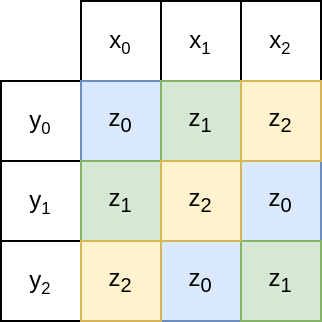
\includegraphics[width=0.9\textwidth]{../resources/cyclic_convolution.drawio.png}
				\caption{Cyclic convolution}
				\label{fig:cyclic_convolution}
		\end{subfigure}%
		\begin{subfigure}{.33\textwidth}
				\centering
				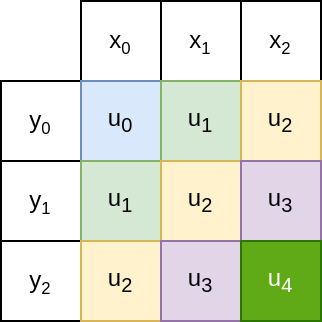
\includegraphics[width=0.9\textwidth]{../resources/acyclic_convolution.drawio.png}
				\caption{Acyclic convolution}
				\label{fig:acyclic_convolution}
		\end{subfigure}%
		\begin{subfigure}{.33\textwidth}
				\centering
				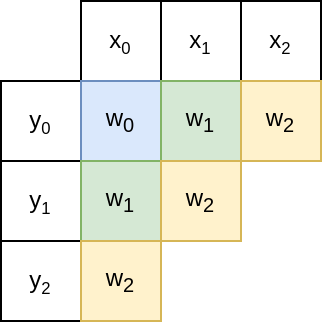
\includegraphics[width=0.9\textwidth]{../resources/halfcyclic_convolution.drawio.png}
				\caption{Halfcyclic convolution}
				\label{fig:halfcyclic_convolution}
		\end{subfigure}
		\begin{subfigure}{.66\textwidth}
				\centering
				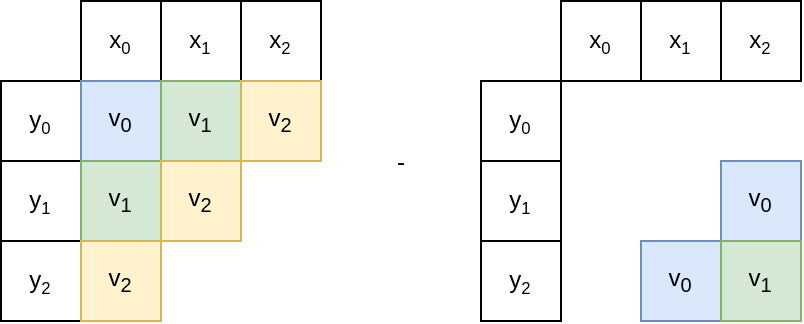
\includegraphics[width=0.9\textwidth]{../resources/negacyclic_convolution.drawio.png}
				\caption{Negacyclic convolution}
				\label{fig:negacyclic_convolution}
		\end{subfigure}
		\caption{
				Different types of discrete convolutions. The input signals $x
				= (x_0, x_1, x_2)$ and $y = (y_0, y_1, y_2)$ are shown along
				the axes. The `cross product' of the input signals represents
				components of the convolution's output, with  labels and
				colours indicating towards which component of the output the
				respective product contributes.  Unless specified otherwise,
				each output signal component is the sum of all products with
				the corresponding label and colour.
}
\end{figure}

\subsection{Relations between convolutions}
\label{sec:relations_between_convolutions}

Various relations between the different types of convolutions exist. One we
will use is the following. Let $L(x)$ be the left half of an even-length
signal. That is if $x = (x_1, x_2, \ldots, x_{2n})$, then $L(x) = (x_1, x_2,
\ldots, x_n)$. Consider now two length-$2n$ signals $x, y$, with the upper half
of either signal being $0$. That is $x_i = y_i = 0, n + 1 \leq i \leq 2n$. Then
it holds that: \autocite{crandallPrimeNumbersComputational2005}

\[
		L(x) \times_A L(y) = x \times y = x \times_\_ y = x \times_H y
\]

These equalities all follow directly from the definition of the convolutions,
using the fact that the upper halves of the input signals are equal to zero.

% Equality of the cyclic and half-cyclic convolution follows directly from their
% definition. They only differ in whether products containing the upper halves of
% the input signals are added to the output signal or not. As the upper halves of
% the input signals are zero however, the two convolutions are equal.
% 
% Equality of the cyclic and negacyclic follows equivalently in that they only
% differ in whether the products containing the upper halves are added or
% subtracted.
% 
% Equality of the half-cyclic of the full and acylic of the lower halves of the
% input signals then follows as seen earlier, in that the half-cyclic is equal to
% the left half of the acyclic of the full.

\subsection{Convolution theorem}
\label{sec:convolution_theorem}

It can further be shown that the cyclic convolution and weighted cyclic
convolution can be calculated by means of the DFT and DWT:
\autocite{crandallPrimeNumbersComputational2005}

\begin{align*}
		x \times y & = \dft^{-1}(\dft(x) \cdot \dft(y)) \\
		x \times_a y & = \dwt^{-1}(\dwt(x, a) \cdot \dwt(y, a), a)
\end{align*}

Where $\cdot$ denotes component-wise multiplication. This allows calculation of
convolutions with complexity $O(n \log(n))$.

By choosing an appropriate weight vector $a$, this also allows the calculation
of other convolutions. Consider choosing the weight vector $a = (a_j) = A^j$
for a scalar $A$. As described by Crandall and Fagin
\autocite{crandallDiscreteWeightedTransforms1994}, the weighted cyclic
convolution of two length-$n$ signals will then take on the following form:

\[
		x \times_a y = (x \times_H y)  + A^n (x \times y - x \times_H y)
\]

Assume then that $A$ is a primitive $2n$-th root of unity. That is $a^{2n} = 1
\Rightarrow a^n = -1$. Then clearly the result of the weighted cyclic
convolution will be the negacyclic convolution:

\[
		x \times_a y = (x \times_H y) - (x \times y - x \times_H y) = 2 \cdot (x \times_H y) - (x \times y) = x \times_\_ y
\]
